\chapter{Configuraci\'on del ambiente de trabajo}
Para trabajar se debe cumplir los requisitos:
\begin{itemize}
	\item Tener instalado Node.
	\item Tener instalado Angular.
	\item Tener instalado Java.
	\item Tener instalado Android Studio.
	\item Tener instalado Visual Code.
	\item Tener bien configurado las variables envolventes.
\end{itemize}
.\\

\section{Instalaci\'on de Node}
Instalaremos  la \'ultima versi\'on de Node.js y npm , recomendamos seleccionar
 la versi\'on LTS para garantizar la mejor compatibilidad . Node se incluye con
  npm, el administrador de paquetes para JavaScript .
Puede descargar el instalador para windows en :\\
\url{https://nodejs.org/es/}\\
\begin{figure}[H] % Ambiente 'figure'
	\centering % imagen sin escalar
	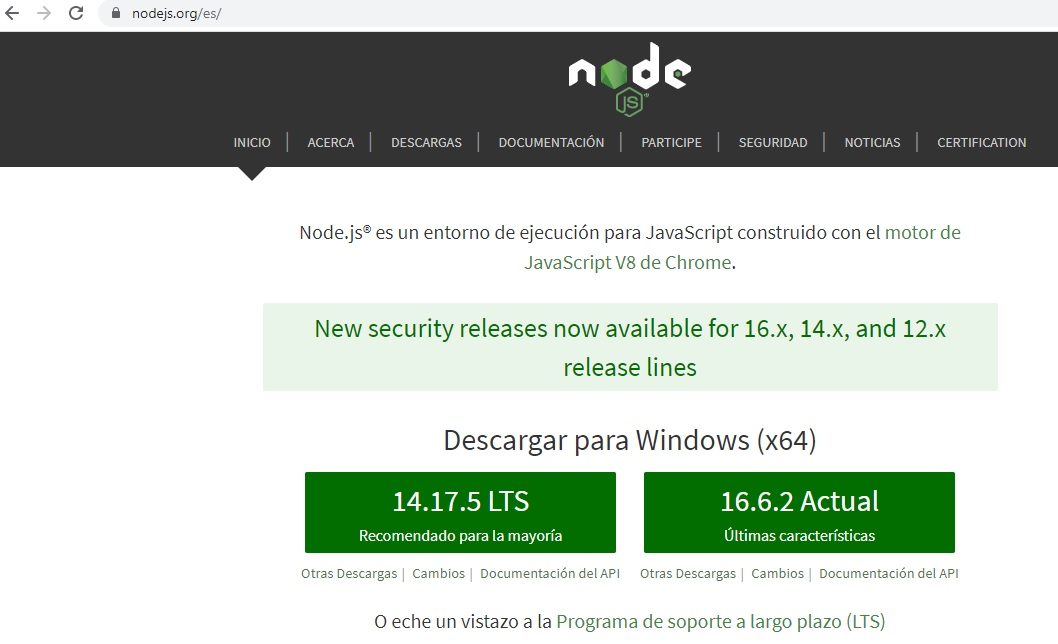
\includegraphics[scale=0.5]{figuras/fig_1_1.jpg}
	\caption{P\'agina web de Node.}
\end{figure}

Abrimos un cmd en modo administrador y nos ubicamos en el directorio donde esta el instalador de node .Ejecutamos la instalaci\'on desde el cmd.
\begin{figure}[H] % Ambiente 'figure'
	\centering % imagen sin escalar
	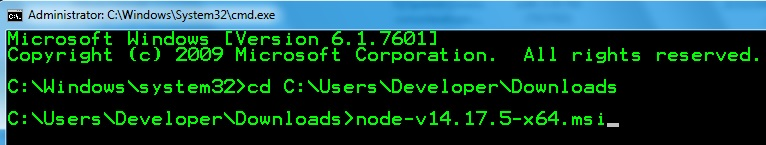
\includegraphics[scale=0.8]{figuras/fig_1_2.jpg}
	\caption{Instalaci\'on de node .}
\end{figure}

 Para verificar  la instalaci\'on, en el cmd terminal de windows  ejecut\'e:\\\\
\texttt{node -v}\\
\texttt{npm -v}\\
\begin{figure}[H] % Ambiente 'figure'
	\centering % imagen sin escalar
	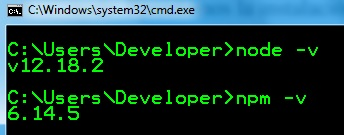
\includegraphics[scale=0.8]{figuras/fig_1_3.jpg}
	\caption{Versi\'on de node y npm.}
\end{figure}


\section{Instalaci\'on de Angular}
Se recomienda tener instalado angular.Para hacer la instalaci\'on  de  angular ejecutar en el cmd. \\\\
\texttt{npm install -g @angular/cli} \\\\
	Para ver la version de angular\\
\texttt{ng version}
\begin{figure}[H] % Ambiente 'figure'
	\centering % imagen sin escalar
	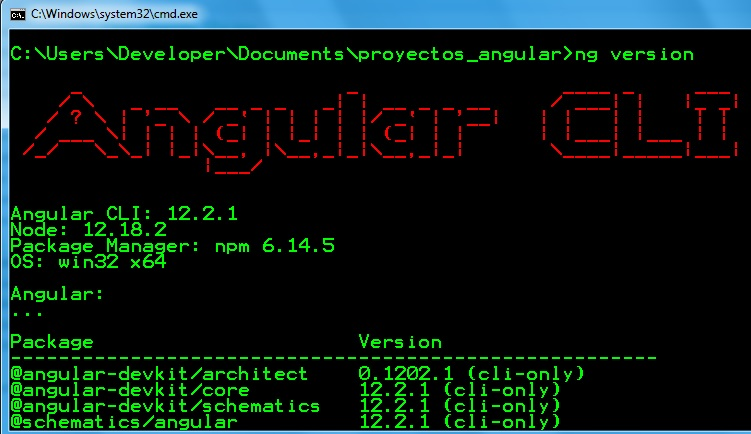
\includegraphics[scale=0.8]{figuras/fig_1_4.jpg}
	\caption{Versi\'on de angular.}
\end{figure}

\section{Instalaci\'on de Ionic}
Las aplicaciones de Ionic se crean y desarrollan principalmente a trav\'es de la utilidad de l\'\i{}nea  de comandos de Ionic. Ionic CLI es el m\'etodo preferido de instalaci\'on, ya que ofrece una amplia gama de herramientas de desarrollo y opciones de ayuda en el camino. Tambi\'en es la herramienta principal para ejecutar la aplicaci\'on y conectarla a otros servicios.\\
Comando para instalar el cliente de ionic ,junto con cordova  (La opci\'on -g significa instalar globalmente).\\
\texttt{npm install -g ionic@latest}\\
\texttt{npm install -g ionic cordova}\\
\texttt{ionic version}
\begin{figure}[H] % Ambiente 'figure'
	\centering % imagen sin escalar
	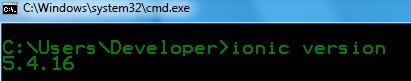
\includegraphics[scale=0.8]{figuras/fig_1_5.jpg}
	\caption{Versi\'on de ionic.}
\end{figure}

\subsection{Instalaciones adicionales para ionic}
Creamos una carpeta con nombre proyectos\_ionic y nos ubicamos en la ruta de la carpeta creada.Ejecutamos los siguientes comandos :\\\\
\texttt{npm install @ionic/app-scripts}

\section{Instalaci\'on de Java}
\section{Instalaci\'on de Android Studio}
\section{Instalaci\'on de Visual Code}


